\begin{figure*}[t]
\centering
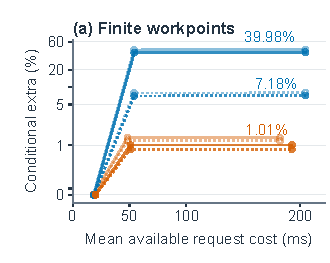
\includegraphics[width=.326\textwidth]{v4_figures/residual_results/opportunity_workpoints.pdf}\hfill
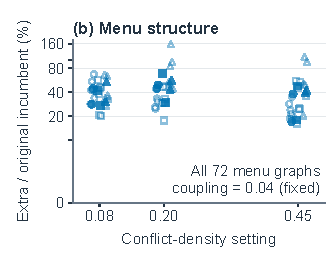
\includegraphics[width=.326\textwidth]{v4_figures/residual_results/opportunity_scenarios.pdf}\hfill
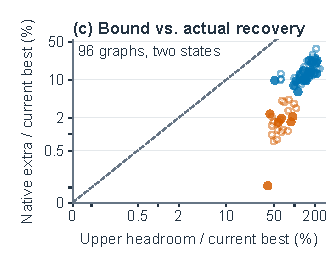
\includegraphics[width=.326\textwidth]{v4_figures/residual_results/opportunity_slack.pdf}

\includegraphics[width=.97\textwidth]{v4_figures/residual_results/opportunity_legend.pdf}
\caption{\textbf{Where additional joint recovery is available.}
Two actual snapshots per development graph.
(a) Best single-call admitted extra versus mean request cost; solid/dotted
curves normalize by original/current incumbents. (b) Menu topology and
density at fixed coupling 0.04. (c) Finite extra versus clique-bound headroom,
normalized by current best; diagonal: equality. Axes are linear near zero,
logarithmic beyond. These are conditional opportunities, not policy gains.}
\label{fig:conditional-recovery-opportunity}
\end{figure*}
